\documentclass{article}
\usepackage{amsmath,amssymb,listings,upquote}
\usepackage[margin=3cm]{geometry}
\usepackage{graphicx,color}
\lstset{language=Python}

\newcounter{zone}
\setcounter{zone}{0}
\newcommand{\zone}{\clearpage\refstepcounter{zone}\section*{Zone \arabic{zone}}}
\newcounter{question}
\setcounter{question}{0}
\newcounter{variant}
\newcounter{questionpoints}
\newcommand{\question}[1]{\newpage \refstepcounter{question} \setcounter{variant}{0} \setcounter{questionpoints}{#1}}
\newcommand{\variant}{\vspace{4em}\refstepcounter{variant}\noindent \arabic{question}/\arabic{variant}. (\arabic{questionpoints} point\ifnum \thequestionpoints > 1 s\fi) }
\newenvironment{answers}{\begin{enumerate}}{\end{enumerate}}
\newcommand{\answer}{\item }
\newcommand{\correctanswer}{\item $\bigstar$ }
\renewcommand{\theenumi}{\Alph{enumi}}
\newenvironment{solution}{{\bf Solution.} }{\vspace*{.3in}\hrule}



\begin{document}
%%%%%%%%%%%%%%%%%%%%%%%%%%%%%%%%%%%%%%%%%%%%%%%%%%%%%%%%%%%%%%%%%%%%%%
%%%%%%%%%%%%%%%%%%%%%%%%%%%%%%%%%%%%%%%%%%%%%%%%%%%%%%%%%%%%%%%%%%%%%%
%%%%%%%%%%%%%%%%%%%%%%%%%%%%%%%%%%%%%%%%%%%%%%%%%%%%%%%%%%%%%%%%%%%%%%
%%%%%%%%%%%%%%%%%%%%%%%%%%%%%%%%%%%%%%%%%%%%%%%%%%%%%%%%%%%%%%%%%%%%%%
% Exam number 1

\message{Exam 1/1}
\cleardoublepage
\setcounter{page}{1}


\begin{center}
\textbf{\Large CS 101 Proficiency Exam \\ Fall 2016}
\end{center}

\bigskip
\noindent
\begin{itemize}
\item \textbf{Be sure to enter your \underline{NetID} and \underline{the code below} on your Scantron}.
\item Do not turn this page until instructed to.
\item There are a total of 200 possible points on this exam.
\item There are 30 multiple choice questions worth 5 points each.
\item There are 2 coding questions worth 25 points each.
\item Each question has only \textbf{one} correct answer.
\item You must not communicate with other students during this test.
\item No books, notes, or electronic devices allowed.
\item This is a 120-minute exam.
\item There are several different versions of this exam.
\end{itemize}

\bigskip\bigskip
\noindent
\textbf{\Large 1. Fill in your information:}

\bigskip
{\Large\bf
\begin{tabular}{ll}
Full Name: & \underbar{\hskip 8cm} \\[0.5em]
UIN (Student Number): & \underbar{\hskip 8cm} \\[0.5em]
NetID: & \underbar{\hskip 8cm}
\end{tabular}
}

\bigskip
\bigskip
\noindent
\textbf{\Large 2. Fill in the following answers on the Scantron form:}

%%%%%%%%%%%%%%%%%%%%%%%%%%%%%%%%%%%%%%%%%%%%%%%%%%%%%%%%%%%%%%%%%%%%%%%%%%%%%%%%
%%%%%%%%%%%%%%%%%%%%%%%%%%%%%%%%%%%%%%%%%%%%%%%%%%%%%%%%%%%%%%%%%%%%%%%%%%%%%%%%

\begin{enumerate}
\item[95.] D
\item[96.] C
\end{enumerate}

\newpage

% Zone 1

\pagebreak \noindent \textbf{The following 20 questions are about Python.}
\\\\
%%%%%%%%%%%%%%%%%%%%%%%%%%%%%%%%%%%%%%%%%%%%%%%%%%%%%%%%%%%%%%%%%%%%%%%%%%%%%%%%
%%%%%%%%%%%%%%%%%%%%%%%%%%%%%%%%%%%%%%%%%%%%%%%%%%%%%%%%%%%%%%%%%%%%%%%%%%%%%%%%


%%%%%%%%%%%%%%%%%%%%%%%%%%%%%%%%%%%%%%%%%%%%%%%%%%%%%%%%%%%%%%%%%%%%%%%%%%%%%%%%



\newpage
\noindent
1. (5 points)
Consider the following simulation program.
\begin{verbatim}
v=500000
x=0.0
t=0.0
dt=.001
while x<1000:
    t+=dt
    x+=v*dt
\end{verbatim}
The program simulates a celestial object moving at constant velocity. Which of the following is a \textbf{state variable} in this simulation?


\begin{enumerate}
\item[(A)]
\begin{verbatim}v\end{verbatim}

\item[(B)] $\bigstar$ 
\begin{verbatim}x\end{verbatim}

\item[(C)]
\begin{verbatim}dt\end{verbatim}

\end{enumerate}

\vspace*{2em}
\hrule
\vspace{2em}

\noindent {\bf Solution.} 
\vspace{2em}
\hrule height 2pt


\newpage
\noindent
2. (5 points)
Consider the following Python program.
\begin{verbatim}
x="1 2 3".split()
x=','.join(x)
try:
    print(x.append(4))
except:
    print(type(x))
\end{verbatim}
After it is run, what is printed by this program?


\begin{enumerate}
\item[(A)]
\begin{verbatim}list\end{verbatim}

\item[(B)] $\bigstar$ 
\begin{verbatim}str\end{verbatim}

\item[(C)]
\begin{verbatim}TypeError\end{verbatim}

\item[(D)]
\begin{verbatim}[1,2,3,4]\end{verbatim}

\end{enumerate}

\vspace*{2em}
\hrule
\vspace{2em}

\noindent {\bf Solution.} 
\vspace{2em}
\hrule height 2pt


\newpage
\noindent
3. (5 points)
Consider the following Python program.
\begin{verbatim}
import numpy as np
x=np.array( [2,3,4] ) * 3 - 1
\end{verbatim}
After it is run, what is the final \textbf{value} of x?


\begin{enumerate}
\item[(A)] $\bigstar$ 
$ \left[ \begin{array}{ccc} 5 & 8 & 11 \\ \end{array} \right] $

\item[(B)]
None of the other answers are correct

\item[(C)]
$ \left[ \begin{array}{ccc} 1 & 2 & 3 \\ 1 & 2 & 3  \\ 1 & 2 & 3  \\ \end{array} \right] $

\item[(D)]
$ \left[ \begin{array}{ccccccccc} 1 & 2 & 3 & 1 & 2 & 3 & 1 & 2 & 3 \\ \end{array} \right] $

\item[(E)]
$ \left[ \begin{array}{c} 5 \\ 8 \\ 11 \\ \end{array} \right] $

\end{enumerate}

\vspace*{2em}
\hrule
\vspace{2em}

\noindent {\bf Solution.} 
\vspace{2em}
\hrule height 2pt


\newpage
\noindent
4. (5 points)
Consider the following incomplete program.
\begin{verbatim}
sum=0
for i in range(0,100):
    ???

\end{verbatim}
The program is intended to sum all of the integers between 1 and 100 (inclusive). What should replace the three question marks to complete the program?


\begin{enumerate}
\item[(A)]
\begin{verbatim}sum+1=sum \end{verbatim}

\item[(B)]
\begin{verbatim}sum=sum+i \end{verbatim}

\item[(C)]
\begin{verbatim}sum=sum+1\end{verbatim}

\item[(D)] $\bigstar$ 
\begin{verbatim}sum=sum+i+1 \end{verbatim}

\end{enumerate}

\vspace*{2em}
\hrule
\vspace{2em}

\noindent {\bf Solution.} 
\vspace{2em}
\hrule height 2pt


\newpage
\noindent
5. (5 points)
Consider the following incomplete function.
\begin{verbatim}
def sum_pairs(A):
    total=0
    ???
    return total
\end{verbatim}
The function takes a single parameter A, which contains a list of floats. The function is intended to return the sum of all pairs of values in the list (with no repeats.) For example, given the list \verb|[1,2,3]|, the function should return \verb|12|, because $(1+2)+(1+3)+(2+3)=12$. What should replace the three question marks to complete the function?


\begin{enumerate}
\item[(A)] $\bigstar$ 
\begin{verbatim}
    for i in range(len(A)):
        for j in range(i+1,len(A)):
            total+=A[i]+A[j]
\end{verbatim}

\item[(B)]
\begin{verbatim}
    for i,j in enumerate(A):
            total+=A[i]+A[j]
\end{verbatim}

\item[(C)]
\begin{verbatim}
    for i in range(len(A)):
        for j in range(len(A)):
            total+=A[i]+A[j]
\end{verbatim}

\item[(D)]
\begin{verbatim}
    for i in itertools.permutations(A):
            total+=i[0]+i[1]
\end{verbatim}

\end{enumerate}

\vspace*{2em}
\hrule
\vspace{2em}

\noindent {\bf Solution.} 
\vspace{2em}
\hrule height 2pt


\newpage
\noindent
6. (5 points)
Consider the following program.
\begin{verbatim}
import numpy as np
x=np.arange(1,4)
np.random.shuffle(x)
print(x)
\end{verbatim}
Which of the following is \emph{not} a possible output for this program?


\begin{enumerate}
\item[(A)]
\begin{verbatim}[2,3,1]\end{verbatim}

\item[(B)]
\begin{verbatim}[3,2,1]\end{verbatim}

\item[(C)] $\bigstar$ 
All of the other answers are possible outputs.

\item[(D)]
\begin{verbatim}[1,2,3]\end{verbatim}

\item[(E)]
\begin{verbatim}[3,1,2]\end{verbatim}

\end{enumerate}

\vspace*{2em}
\hrule
\vspace{2em}

\noindent {\bf Solution.} 
\vspace{2em}
\hrule height 2pt


\newpage
\noindent
7. (5 points)
Consider the following Python program.
\begin{verbatim}
e=[1,1,2,2,3,3,4,4,5,5,6,6]
d={0:0,1:0,2:0}
for a,b in enumerate(e):
    d[a%3]+=b
x=d[1]
\end{verbatim}
After it is run, what is the final \textbf{value} of x?


\begin{enumerate}
\item[(A)]
\begin{verbatim}12\end{verbatim}

\item[(B)]
\begin{verbatim}3\end{verbatim}

\item[(C)]
\begin{verbatim}22\end{verbatim}

\item[(D)]
\begin{verbatim}8\end{verbatim}

\item[(E)] $\bigstar$ 
\begin{verbatim}14\end{verbatim}

\end{enumerate}

\vspace*{2em}
\hrule
\vspace{2em}

\noindent {\bf Solution.} 
\vspace{2em}
\hrule height 2pt


\newpage
\noindent
8. (5 points)
Consider the following incomplete Python program.
\begin{verbatim}
s="".join(["2","2","0","1","2"])
x=0
for i in range(len(s)-1):
    x+=int(???)
\end{verbatim}
What should replace the three question marks so the resulting value of x is 55?


\begin{enumerate}
\item[(A)] $\bigstar$ 
\begin{verbatim}s[i:i+2]\end{verbatim}

\item[(B)]
\begin{verbatim}s[i:i-1]\end{verbatim}

\item[(C)]
\begin{verbatim}s[i+1:i+2]\end{verbatim}

\item[(D)]
\begin{verbatim}s[i:i+1]\end{verbatim}

\end{enumerate}

\vspace*{2em}
\hrule
\vspace{2em}

\noindent {\bf Solution.} 
\vspace{2em}
\hrule height 2pt


\newpage
\noindent
9. (5 points)
Consider the following incomplete Python function.
\begin{verbatim}
def total_sales(sales_file):
    d={}
    for line in open(sales_file):
        ???
    return d
\end{verbatim}
The function is intended to compute the total sales of each employee working for a company by reading a comma separated (csv) input file of employee sale data. The result should be stored in a dictionary. The first column of each line in the input file is expected to contain the employee's name represented as a string. The second column is expected to contain a floating point number representing the total for that sale. Here is an example input file:
\begin{verbatim}
Bob,10.0
Jill,10.55
Jill,115.50
Your program should ignore this line
Bob,30.25
\end{verbatim}
The resulting return value for this file should be the following dictionary:
\begin{verbatim}
{'Bob': 40.25, 'Jill': 126.05}
\end{verbatim}
What should replace the three question marks to complete the function?


\begin{enumerate}
\item[(A)]
\begin{verbatim}
try:
    s,f=line.split(",")
except:
    continue
if f not in d:
    d[f]=0.0
d[f]+=float(s)
\end{verbatim}

\item[(B)]
\begin{verbatim}
if line not in d:
    d[line]=0.0
try:
    s,f=line.split(",")
except:
    d[s]+=float(f)
    continue
\end{verbatim}

\item[(C)] $\bigstar$ 
\begin{verbatim}
try:
    s,f=line.split(",")
    if s not in d:
        d[s]=0.0
    d[s]+=float(f)
except:
    continue
\end{verbatim}

\end{enumerate}

\vspace*{2em}
\hrule
\vspace{2em}

\noindent {\bf Solution.} 
\vspace{2em}
\hrule height 2pt


\newpage
\noindent
10. (5 points)
Consider the following incomplete program.

\begin{verbatim}
import matplotlib.pyplot as plt
import numpy as np
???
plt.hist(x,bins=100)
plot.show()
\end{verbatim}

Which line should replace the three question marks to produce the following plot?

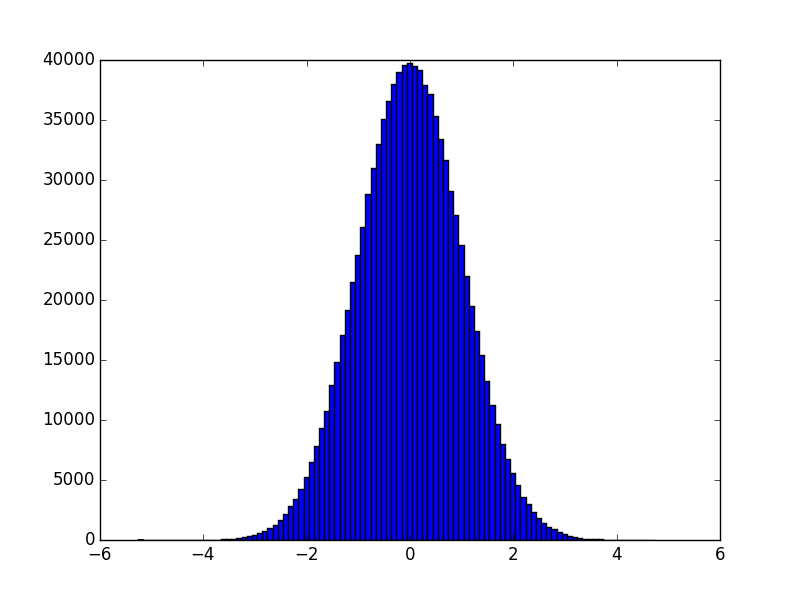
\includegraphics[scale=.5]{./img/normal.png}


\begin{enumerate}
\item[(A)]
\begin{verbatim}x=np.random.shuffle(np.arange(1000000))\end{verbatim}

\item[(B)]
\begin{verbatim}x=np.random.choice(np.arange(1000000))\end{verbatim}

\item[(C)]
\begin{verbatim}x=np.random.rand(1000000)\end{verbatim}

\item[(D)] $\bigstar$ 
\begin{verbatim}x=np.random.randn(1000000)\end{verbatim}

\end{enumerate}

\vspace*{2em}
\hrule
\vspace{2em}

\noindent {\bf Solution.} 
\vspace{2em}
\hrule height 2pt


\newpage
\noindent
11. (5 points)
What do we call the optimization heuristic that involves choosing the best from a stochastically sampled subset of the domain?


\begin{enumerate}
\item[(A)]
Brute-force search

\item[(B)]
Gradient descent

\item[(C)] $\bigstar$ 
Random search

\item[(D)]
Local optimum

\end{enumerate}

\vspace*{2em}
\hrule
\vspace{2em}

\noindent {\bf Solution.} 
\vspace{2em}
\hrule height 2pt


\newpage
\noindent
12. (5 points)
Consider the following program:
\begin{verbatim}
a=["B","I","L","G","E"]
a.sort()
a[0]=a[-1]
x=""
for e in a:
    x=x+e
\end{verbatim}
What is the \textbf{value} of x after this program is executed?


\begin{enumerate}
\item[(A)]
None of the other answers are correct.

\item[(B)] $\bigstar$ 
\begin{verbatim}"LEGIL"\end{verbatim}

\item[(C)]
\begin{verbatim}"BILEB"\end{verbatim}

\item[(D)]
\begin{verbatim}"GILEG"\end{verbatim}

\item[(E)]
\begin{verbatim}"BILGB"\end{verbatim}

\end{enumerate}

\vspace*{2em}
\hrule
\vspace{2em}

\noindent {\bf Solution.} 
\vspace{2em}
\hrule height 2pt


\newpage
\noindent
13. (5 points)
Consider the following incomplete Python program.
\begin{verbatim}
a="HAMBUG"
b="BUSHWA"
d={}
for x,y in zip(a,b):
    ???
s=""
for c in b:
    s+=d[c]
print(s)
\end{verbatim}
Which of the following could replace the three question marks to cause this program to print out  \begin{verbatim}HAMBUG\end{verbatim}?


\begin{enumerate}
\item[(A)]
\begin{verbatim}d[a]=x\end{verbatim}

\item[(B)]
\begin{verbatim}d[a]=b\end{verbatim}

\item[(C)]
\begin{verbatim}d[x]=y\end{verbatim}

\item[(D)] $\bigstar$ 
\begin{verbatim}d[y]=x\end{verbatim}

\item[(E)]
\begin{verbatim}d[b]=a\end{verbatim}

\end{enumerate}

\vspace*{2em}
\hrule
\vspace{2em}

\noindent {\bf Solution.} 
\vspace{2em}
\hrule height 2pt


\newpage
\noindent
14. (5 points)
Consider the following incomplete program.
\begin{verbatim}
v=0.0
y=1.0
g=-9.8
t=0.0
dt=???
while y>0.0:
    t+=dt
    v+=g*dt
    y+=v*dt
\end{verbatim}
The program is intended to simulate an object falling from a height of 1 meter. If we replace the question marks with one of the following values, which choice would produce the most \textit{accurate} simulation?


\begin{enumerate}
\item[(A)] $\bigstar$ 
\begin{verbatim}0.0001\end{verbatim}

\item[(B)]
\begin{verbatim}0.1\end{verbatim}

\item[(C)]
\begin{verbatim}0.01\end{verbatim}

\item[(D)]
\begin{verbatim}0.001\end{verbatim}

\end{enumerate}

\vspace*{2em}
\hrule
\vspace{2em}

\noindent {\bf Solution.} 
\vspace{2em}
\hrule height 2pt


\newpage
\noindent
15. (5 points)
Consider the following program:
\begin{verbatim}
x=["snip","snap"]
x[0]=len(x[1])
if x[0]<4:
    x="A"
\end{verbatim}
What is the \textbf{type} of x after the program is run?


\begin{enumerate}
\item[(A)] $\bigstar$ 
List

\item[(B)]
None

\item[(C)]
String

\item[(D)]
Integer

\item[(E)]
None of the other answers are correct.

\end{enumerate}

\vspace*{2em}
\hrule
\vspace{2em}

\noindent {\bf Solution.} 
\vspace{2em}
\hrule height 2pt


\newpage
\noindent
16. (5 points)
Consider the following incomplete program:
\begin{verbatim}
import itertools
x="HAVER"
???:
    print(x)
\end{verbatim}
Replacing the three question marks with which of the following will result in \begin{verbatim}'HAVER'\end{verbatim} being printed exactly five times?


\begin{enumerate}
\item[(A)]
\begin{verbatim}
for a in itertools.combinations(x,2)
\end{verbatim}

\item[(B)] $\bigstar$ 
\begin{verbatim}
for a in itertools.combinations(x,4)
\end{verbatim}

\item[(C)]
\begin{verbatim}
for a in itertools.combinations(x,5)
\end{verbatim}

\item[(D)]
\begin{verbatim}
for a in itertools.combinations(x,3)
\end{verbatim}

\end{enumerate}

\vspace*{2em}
\hrule
\vspace{2em}

\noindent {\bf Solution.} 
\vspace{2em}
\hrule height 2pt


\newpage
\noindent
17. (5 points)
Consider the following program.
\begin{verbatim}
y=1
for i in range(0,3):
    y=y+(2*y)
x=y>10
\end{verbatim}
After it is run, what is the final \textbf{value} of x?


\begin{enumerate}
\item[(A)]
False

\item[(B)] $\bigstar$ 
True

\end{enumerate}

\vspace*{2em}
\hrule
\vspace{2em}

\noindent {\bf Solution.} 
\vspace{2em}
\hrule height 2pt


\newpage
\noindent
18. (5 points)
Consider the following program:
\begin{verbatim}
a=1
def fun(a):
    a=2
    return a+1
    a=4
fun(a)
print(a)
\end{verbatim}
What is printed out by this program?


\begin{enumerate}
\item[(A)]
2

\item[(B)]
None of the other answers. This code is not valid.

\item[(C)] $\bigstar$ 
1

\item[(D)]
3

\item[(E)]
4

\end{enumerate}

\vspace*{2em}
\hrule
\vspace{2em}

\noindent {\bf Solution.} 
\vspace{2em}
\hrule height 2pt


\newpage
\noindent
19. (5 points)
Consider the following incomplete Python program:
\begin{verbatim}
x=[ ]
for i in range(1,101):
    for j in range(i+1,101):
        t=i,j
        x.append(t)
\end{verbatim}
After the program runs, which of the following is an element of x?


\begin{enumerate}
\item[(A)]
\begin{verbatim}(78,78)\end{verbatim}

\item[(B)]
\begin{verbatim}(0,33)\end{verbatim}

\item[(C)] $\bigstar$ 
\begin{verbatim}(10,52)\end{verbatim}

\item[(D)]
\begin{verbatim}(42,15)\end{verbatim}

\item[(E)]
\begin{verbatim}(11,4)\end{verbatim}

\end{enumerate}

\vspace*{2em}
\hrule
\vspace{2em}

\noindent {\bf Solution.} 
\vspace{2em}
\hrule height 2pt


\newpage
\noindent
20. (5 points)
Consider the following program:
\begin{verbatim}
s="BABOONERY"
x=""
for i in range(0,len(s)):
    if (i>3) and (i<6):
        x+=s[i:i+2]
\end{verbatim}
What is the \textbf{value} of x after this program is executed?


\begin{enumerate}
\item[(A)]
\begin{verbatim}"NE"\end{verbatim}

\item[(B)] $\bigstar$ 
\begin{verbatim}"ONNE"\end{verbatim}

\item[(C)]
\begin{verbatim}"OO"\end{verbatim}

\item[(D)]
None of the other answers are correct.

\item[(E)]
\begin{verbatim}"OOON"\end{verbatim}

\end{enumerate}

\vspace*{2em}
\hrule
\vspace{2em}

\noindent {\bf Solution.} 
\vspace{2em}
\hrule height 2pt

% Zone 2

\pagebreak  \noindent \textbf{The following 10 questions are about MATLAB.}
\\\\
%%%%%%%%%%%%%%%%%%%%%%%%%%%%%%%%%%%%%%%%%%%%%%%%%%%%%%%%%%%%%%%%%%%%%%%%%%%%%%%%
%%%%%%%%%%%%%%%%%%%%%%%%%%%%%%%%%%%%%%%%%%%%%%%%%%%%%%%%%%%%%%%%%%%%%%%%%%%%%%%%

%%%%%%%%%%%%%%%%%%%%%%%%%%%%%%%%%%%%%%%%%%%%%%%%%%%%%%%%%%%%%%%%%%%%%%%%%%%%%%%%



\newpage
\noindent
21. (5 points)
Consider the following MATLAB program.
\begin{verbatim}
A=eye(3,3);
for x=2:1:3
    A(x,x)=0;
end
\end{verbatim}
After it is run, what is the final \textbf{value} of A?


\begin{enumerate}
\item[(A)]
$ \left[ \begin{array}{ccc} 0 & 0 & 0 \\ 0 & 0 & 0 \\ 0 & 0 & 0 \\ \end{array} \right] $

\item[(B)]
$ \left[ \begin{array}{ccc} 1 & 0 & 0 \\ 0 & 1 & 0 \\ 0 & 0 & 1 \\ \end{array} \right] $

\item[(C)] $\bigstar$ 
$ \left[ \begin{array}{ccc} 1 & 0 & 0 \\ 0 & 0 & 0 \\ 0 & 0 & 0 \\ \end{array} \right] $

\item[(D)]
$ \left[ \begin{array}{ccc} 1 & 0 & 1 \\ 0 & 1 & 0 \\ 1 & 0 & 1 \\ \end{array} \right] $

\item[(E)]
$ \left[ \begin{array}{ccc} 0 & 0 & 0 \\ 0 & 1 & 0 \\ 0 & 0 & 0 \\ \end{array} \right] $

\end{enumerate}

\vspace*{2em}
\hrule
\vspace{2em}

\noindent {\bf Solution.} 
\vspace{2em}
\hrule height 2pt


\newpage
\noindent
22. (5 points)
Consider the following MATLAB program.
\begin{verbatim}
A=[3,2,1;0,2,1;0,0,1];
B=(2*eye(3,3)*A)-A;
x=B(1,1)+B(2,2)+B(3);
\end{verbatim}
After it is run, what is the final \textbf{value} of x?


\begin{enumerate}
\item[(A)]
2

\item[(B)] $\bigstar$ 
5

\item[(C)]
6

\item[(D)]
3

\item[(E)]
1

\end{enumerate}

\vspace*{2em}
\hrule
\vspace{2em}

\noindent {\bf Solution.} 
\vspace{2em}
\hrule height 2pt


\newpage
\noindent
23. (5 points)
Consider the following MATLAB program.
\begin{verbatim}
x=3:2:7;
y=4:2:8;
z=x+y;
\end{verbatim}
After it is run, what is the final \textbf{value} of z?


\begin{enumerate}
\item[(A)]
$ \left[ \begin{array}{ccc} 3 & 5 & 7 \\ 4 & 6 & 8 \\ \end{array} \right] $

\item[(B)]
$ \left[ \begin{array}{ccccc} 7 & 11 \\ \end{array} \right] $

\item[(C)] $\bigstar$ 
$ \left[ \begin{array}{ccccc} 7 & 11 & 15 \\ \end{array} \right] $

\item[(D)]
$ \left[ \begin{array}{ccc} 3 & 2 & 7 \\ 4 & 2 & 8 \\ \end{array} \right] $

\item[(E)]
$ \left[ \begin{array}{cc} 3 & 7 \\ 4 & 8 \\ \end{array} \right] $

\end{enumerate}

\vspace*{2em}
\hrule
\vspace{2em}

\noindent {\bf Solution.} 
\vspace{2em}
\hrule height 2pt


\newpage
\noindent
24. (5 points)
Consider the following MATLAB program.
\begin{verbatim}
A=[1,1,1;0,1,1;0,0,1];
B=A';
x=B(1,1)+B(2,2)+B(3,3);
\end{verbatim}
After it is run, what is the final \textbf{value} of x?


\begin{enumerate}
\item[(A)]
2

\item[(B)]
1

\item[(C)]
None of the other answers are correct.

\item[(D)]
0

\item[(E)] $\bigstar$ 
3

\end{enumerate}

\vspace*{2em}
\hrule
\vspace{2em}

\noindent {\bf Solution.} 
\vspace{2em}
\hrule height 2pt


\newpage
\noindent
25. (5 points)
Consider the following MATLAB program.
\begin{verbatim}
A=eye(3,3)+ones(3,3);
for x=1:3
    for y=1:3
        if x>y
            A(x,y)=x+y;
        end
    end
end
\end{verbatim}
After it is run, what is the final \textbf{value} of A?


\begin{enumerate}
\item[(A)]
$ \left[ \begin{array}{ccc} 2 & 3 & 4 \\ 1 & 2 & 5 \\ 1 & 1 & 2  \\ \end{array} \right] $

\item[(B)]
$ \left[ \begin{array}{ccc} 2 & 1 & 1 \\ 3 & 4 & 1 \\ 4 & 4 & 6 \\ \end{array} \right] $

\item[(C)]
$ \left[ \begin{array}{ccc} 2 & 3 & 4 \\ 1 & 4 & 5 \\ 1 & 1 & 6  \\ \end{array} \right] $

\item[(D)] $\bigstar$ 
$ \left[ \begin{array}{ccc} 2 & 1 & 1 \\ 3 & 2 & 1 \\ 4 & 5 & 2 \\ \end{array} \right] $

\end{enumerate}

\vspace*{2em}
\hrule
\vspace{2em}

\noindent {\bf Solution.} 
\vspace{2em}
\hrule height 2pt


\newpage
\noindent
26. (5 points)
Consider the following MATLAB program.
\begin{verbatim}
A=[[ones(2,2),[2;2]];3,3,3];
x=A(2,3);
\end{verbatim}
After it is run, what is the final \textbf{value} of x?


\begin{enumerate}
\item[(A)] $\bigstar$ 
2

\item[(B)]
3

\item[(C)]
0

\item[(D)]
1

\end{enumerate}

\vspace*{2em}
\hrule
\vspace{2em}

\noindent {\bf Solution.} 
\vspace{2em}
\hrule height 2pt


\newpage
\noindent
27. (5 points)
Consider the following MATLAB program.
\begin{verbatim}
x=[1,2];
y=[3,4];
z=[y,x;x,y]';
\end{verbatim}
After it is run, what is the final \textbf{value} of z?


\begin{enumerate}
\item[(A)]
$ \left[ \begin{array}{cccc} 3 & 4 & 1 & 2\\ 1 & 2 & 3 & 4 \\ \end{array} \right] $

\item[(B)]
None of the other answers are correct

\item[(C)] $\bigstar$ 
$ \left[ \begin{array}{cc} 3 & 1 \\ 4 & 2 \\ 1 & 3 \\ 2 & 4 \\ \end{array} \right] $

\item[(D)]
$ \left[ \begin{array}{cc} 1 & 3 \\ 2 & 4 \\ 3 & 1 \\ 4 & 2 \\ \end{array} \right] $

\item[(E)]
$ \left[ \begin{array}{cccc} 1 & 2 & 3 & 4\\ 3 & 4 & 1 & 2 \\ \end{array} \right] $

\end{enumerate}

\vspace*{2em}
\hrule
\vspace{2em}

\noindent {\bf Solution.} 
\vspace{2em}
\hrule height 2pt


\newpage
\noindent
28. (5 points)
Consider the following MATLAB program.
\begin{verbatim}
x=(3<5) && (2>3)
\end{verbatim}
After it is run, what is the final \textbf{value} of x?


\begin{enumerate}
\item[(A)]
True

\item[(B)] $\bigstar$ 
0

\item[(C)]
1

\item[(D)]
False

\end{enumerate}

\vspace*{2em}
\hrule
\vspace{2em}

\noindent {\bf Solution.} 
\vspace{2em}
\hrule height 2pt


\newpage
\noindent
29. (5 points)
Consider the following 2-dimensional MATLAB array:

$ \left[ \begin{array}{ccc} 1 & 2 & 3 \\ 4 & 5 & 6 \\ 7 & 8 & 9 \\ 10 & 11 & 12 \\ \end{array} \right] $ \\

Assuming it is stored in a variable named A, how can we index and retrieve the value 8?


\begin{enumerate}
\item[(A)]
A(2,3)

\item[(B)] $\bigstar$ 
A(3,2)

\item[(C)]
A(1,2)

\item[(D)]
A(2,1)

\end{enumerate}

\vspace*{2em}
\hrule
\vspace{2em}

\noindent {\bf Solution.} 
\vspace{2em}
\hrule height 2pt


\newpage
\noindent
30. (5 points)
Consider the following MATLAB program.
\begin{verbatim}
x=[2;3;4];
x=3*eye(3,3)*x;
x=x(1)+x(2)+x(3)
\end{verbatim}
After it is run, what is the final \textbf{value} of x?


\begin{enumerate}
\item[(A)] $\bigstar$ 
27

\item[(B)]
The program contains a syntax error and will not run.

\item[(C)]
12

\item[(D)]
9

\item[(E)]
6

\end{enumerate}

\vspace*{2em}
\hrule
\vspace{2em}

\noindent {\bf Solution.} 
\vspace{2em}
\hrule height 2pt

% Zone 3

\pagebreak \noindent \textbf{The following 2 coding questions are about Python.}
\\\\
\noindent Be sure to write clearly and comment your code, so we can understand your answer.
\\\\
%%%%%%%%%%%%%%%%%%%%%%%%%%%%%%%%%%%%%%%%%%%%%%%%%%%%%%%%%%%%%%%%%%%%%%%%%%%%%%%%
%%%%%%%%%%%%%%%%%%%%%%%%%%%%%%%%%%%%%%%%%%%%%%%%%%%%%%%%%%%%%%%%%%%%%%%%%%%%%%%%



\newpage
\noindent
31. (25 points)
Your friend Vanessa can't remember her Facebook password and wants your help figuring it out. She remembers the password is exactly 9 characters long. She also remembers that her username is either ``vanessa'' or ``VanessaC'' or ``Vanessa95''. Assume someone else has already written a function \verb|login| that takes a two string arguments representing a username and password combination. \verb|login| returns  \verb|True| if the input username and password are valid credentials for Facebook and \verb|False| otherwise. Your function  \verb|guess_password| should perform a brute force search and return the correct username and password for Vanessa's account as a tuple of two strings.
\\\\
\noindent We set up the alphabet string for you. Assume all of the possible password characters are contained in this string. You may import itertools in your solution if you prefer, but no other libraries are allowed.

\begin{verbatim}
def guess_password():
    alphabet="ABCDEFGHIJKLMNOPQRSTUVWXYZabcdefghijklmnopqrstuvwxyz"
    alphabet+="0123456789!@#$%^&*()-_=+,<.>/?~`"
\end{verbatim}


\vspace*{2em}
\hrule
\vspace{2em}

\noindent {\bf Solution.} 
\vspace{2em}
\hrule height 2pt

% Zone 4

\pagebreak \noindent




\newpage
\noindent
32. (25 points)
Write a Python program to simulate a population of rabbits for 50 years. Your simulation should update annually (i.e. $\Delta t=1$ year). The initial population of rabbits is 15. Each year, 5\% of the population of the previous year dies off, and each year exactly 5 new rabbits are born. In your simulation, it should be impossible for ``partial rabbits'' to exist. For example, the population should never be 13.7. 70\% of a rabbit is a grisly idea, and it's probably best that we don't spend any more time thinking about it. You should always round the population \emph{down} to a whole number.
\\\\
\noindent You may import NumPy in your solution if you prefer, but no other libraries are allowed.


\vspace*{2em}
\hrule
\vspace{2em}

\noindent {\bf Solution.} 
\vspace{2em}
\hrule height 2pt

\end{document}
